\documentclass[aspectratio=169]{beamer}

\usetheme{Boadilla}
\usecolortheme{dolphin}
\usefonttheme{professionalfonts}

\usepackage[utf8]{inputenc}
\usepackage[T1]{fontenc}
\usepackage{lmodern}
\usepackage{tikz}
\usepackage{listings}
\usepackage{xcolor}
\usetikzlibrary{arrows.meta,positioning,calc,shapes.geometric}

\definecolor{Ink}{HTML}{111827}
\definecolor{Night}{HTML}{172033}
\definecolor{Blue}{HTML}{2563EB}
\definecolor{Green}{HTML}{22C55E}
\definecolor{Red}{HTML}{EF4444}
\definecolor{Yellow}{HTML}{FACC15}
\definecolor{Violet}{HTML}{7C3AED}
\definecolor{Soft}{HTML}{F7F4EF}

\setbeamercolor{normal text}{fg=Ink,bg=Soft}
\setbeamercolor{frametitle}{fg=white,bg=Night}
\setbeamercolor{title}{fg=white,bg=Night}
\setbeamercolor{block title}{fg=white,bg=Blue}
\setbeamercolor{block body}{fg=Ink,bg=white}
\setbeamertemplate{navigation symbols}{}

\lstdefinelanguage{JavaScript}{
  morekeywords={let,const,var,function,if,else,for,of,return,true,false,null,new,break},
  sensitive=true,
  morecomment=[l]{//},
  morestring=[b]",
  morestring=[b]'
}

\lstdefinestyle{jsstyle}{
  language=JavaScript,
  basicstyle=\ttfamily\small,
  keywordstyle=\color{Blue}\bfseries,
  stringstyle=\color{Green!55!black},
  commentstyle=\color{Ink!55},
  numberstyle=\tiny\color{Ink!45},
  numbers=left,
  stepnumber=1,
  numbersep=8pt,
  showstringspaces=false,
  tabsize=2,
  breaklines=true,
  frame=single,
  rulecolor=\color{Ink!20},
  backgroundcolor=\color{white}
}

\newcommand{\player}[2]{
  \begin{scope}[shift={(#1,#2)}]
    \draw[fill=Green, draw=white, line width=1.2pt] (0,0) circle (0.32);
    \draw[white, line width=2.2pt, -{Latex[length=3mm]}] (0,0) -- (0.62,0);
    \fill[Ink!70] (0.12,0.1) circle (0.04);
  \end{scope}
}

\newcommand{\enemy}[2]{
  \begin{scope}[shift={(#1,#2)}]
    \draw[fill=Red, draw=white, line width=1pt] (0,0) circle (0.26);
    \fill[Ink!60] (0.08,0.08) circle (0.04);
  \end{scope}
}

\newcommand{\shot}[2]{
  \fill[Yellow] (#1,#2) circle (0.08);
}

\title{Dal ciclo al videogioco}
\subtitle{Laboratorio JavaScript: costruiamo un mini shooter}
\author{Game Design Summer School 2026}
\date{}

\begin{document}

\begin{frame}
  \titlepage
  \begin{tikzpicture}[remember picture,overlay]
    \fill[Blue] ($(current page.south west)+(0,0)$) rectangle ($(current page.south east)+(16,0.15)$);
    \fill[Green] ($(current page.south west)+(0,0.15)$) rectangle ($(current page.south west)+(5.3,0.3)$);
    \fill[Yellow] ($(current page.south west)+(5.3,0.15)$) rectangle ($(current page.south west)+(10.6,0.3)$);
    \fill[Red] ($(current page.south west)+(10.6,0.15)$) rectangle ($(current page.south east)+(16,0.3)$);
  \end{tikzpicture}
\end{frame}

\begin{frame}{Obiettivo del laboratorio}
  \begin{columns}[T]
    \begin{column}{0.54\textwidth}
      \begin{block}{Alla fine sappiamo spiegare}
        \begin{itemize}
          \item che cosa e' un ciclo;
          \item perche' un gioco aggiorna lo schermo molte volte;
          \item come tastiera, posizione e velocita' diventano regole;
          \item come array e collisioni creano il gameplay.
        \end{itemize}
      \end{block}
    \end{column}
    \begin{column}{0.42\textwidth}
      \centering
      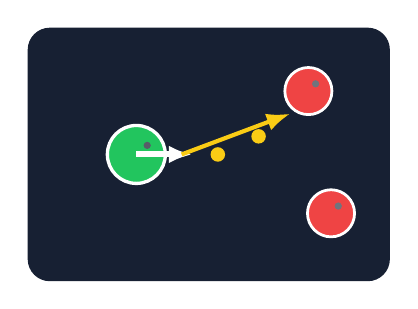
\begin{tikzpicture}[scale=1.15]
        \fill[Night, rounded corners=8pt] (-2,-1.4) rectangle (2,1.4);
        \player{-0.8}{0}
        \enemy{1.1}{0.7}
        \enemy{1.35}{-0.65}
        \shot{0.1}{0}
        \shot{0.55}{0.2}
        \draw[Yellow, line width=1.5pt, -{Latex[length=3mm]}] (-0.3,0) -- (0.9,0.45);
      \end{tikzpicture}
    \end{column}
  \end{columns}
\end{frame}

\begin{frame}{La mappa degli step}
  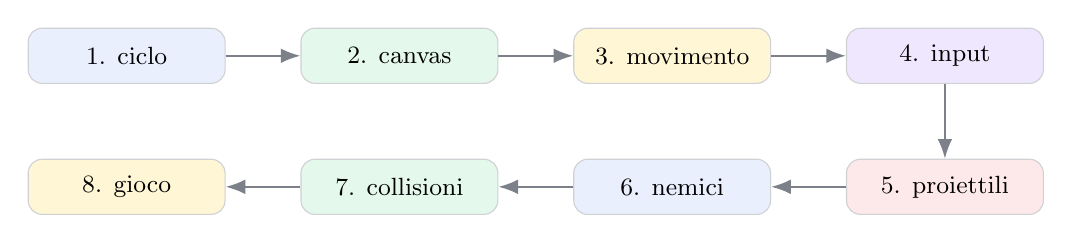
\begin{tikzpicture}[
    node distance=0.95cm,
    box/.style={draw=Ink!20, fill=white, rounded corners=5pt, minimum width=2.5cm, minimum height=0.7cm, align=center, font=\small},
    arrow/.style={-{Latex[length=2.5mm]}, thick, draw=Ink!55}
  ]
    \node[box, fill=Blue!10] (a) {1. ciclo};
    \node[box, right=of a, fill=Green!12] (b) {2. canvas};
    \node[box, right=of b, fill=Yellow!18] (c) {3. movimento};
    \node[box, right=of c, fill=Violet!12] (d) {4. input};
    \node[box, below=of d, fill=Red!12] (e) {5. proiettili};
    \node[box, left=of e, fill=Blue!10] (f) {6. nemici};
    \node[box, left=of f, fill=Green!12] (g) {7. collisioni};
    \node[box, left=of g, fill=Yellow!18] (h) {8. gioco};

    \draw[arrow] (a) -- (b);
    \draw[arrow] (b) -- (c);
    \draw[arrow] (c) -- (d);
    \draw[arrow] (d) -- (e);
    \draw[arrow] (e) -- (f);
    \draw[arrow] (f) -- (g);
    \draw[arrow] (g) -- (h);
  \end{tikzpicture}
\end{frame}

\begin{frame}[fragile]{Step 1: un ciclo nel tempo}
  \begin{columns}[T]
    \begin{column}{0.52\textwidth}
      \begin{lstlisting}[style=jsstyle]
function setup() {
  let volte = 0;

  setInterval(() => {
    volte = volte + 1;
    log("tick " + volte);
  }, 500);
}
      \end{lstlisting}
    \end{column}
    \begin{column}{0.42\textwidth}
      \begin{block}{Idea chiave}
        Un gioco non fa una sola cosa: ripete continuamente piccole azioni.
      \end{block}
      \vspace{0.2cm}
      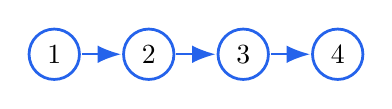
\begin{tikzpicture}
        \foreach \x/\t in {0/1,1.2/2,2.4/3,3.6/4} {
          \draw[fill=white, draw=Blue, line width=1pt] (\x,0) circle (0.32);
          \node at (\x,0) {\t};
        }
        \draw[Blue, thick, -{Latex[length=3mm]}] (0.35,0) -- (0.85,0);
        \draw[Blue, thick, -{Latex[length=3mm]}] (1.55,0) -- (2.05,0);
        \draw[Blue, thick, -{Latex[length=3mm]}] (2.75,0) -- (3.25,0);
      \end{tikzpicture}
    \end{column}
  \end{columns}
\end{frame}

\begin{frame}{Il game loop}
  \centering
  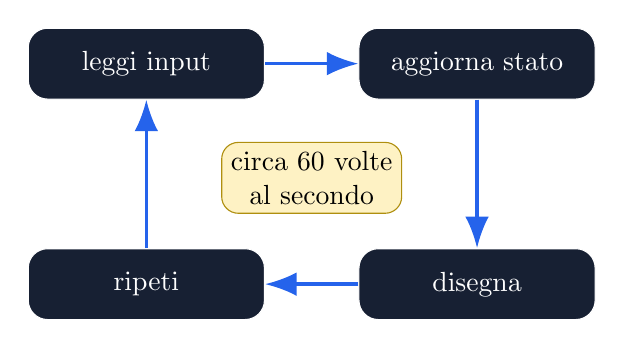
\begin{tikzpicture}[
    block/.style={draw=white, fill=Night, text=white, rounded corners=7pt, minimum width=3cm, minimum height=0.9cm, align=center},
    arrow/.style={-{Latex[length=4mm]}, line width=1.2pt, draw=Blue}
  ]
    \node[block] (input) at (0,1.8) {leggi input};
    \node[block] (update) at (4.2,1.8) {aggiorna stato};
    \node[block] (draw) at (4.2,-1.0) {disegna};
    \node[block] (repeat) at (0,-1.0) {ripeti};

    \draw[arrow] (input) -- (update);
    \draw[arrow] (update) -- (draw);
    \draw[arrow] (draw) -- (repeat);
    \draw[arrow] (repeat) -- (input);

    \node[fill=Yellow!25, draw=Yellow!70!black, rounded corners=6pt, align=center] at (2.1,0.35)
      {circa 60 volte\\al secondo};
  \end{tikzpicture}
\end{frame}

\begin{frame}{Coordinate: la mappa dello schermo}
  \begin{columns}[T]
    \begin{column}{0.55\textwidth}
      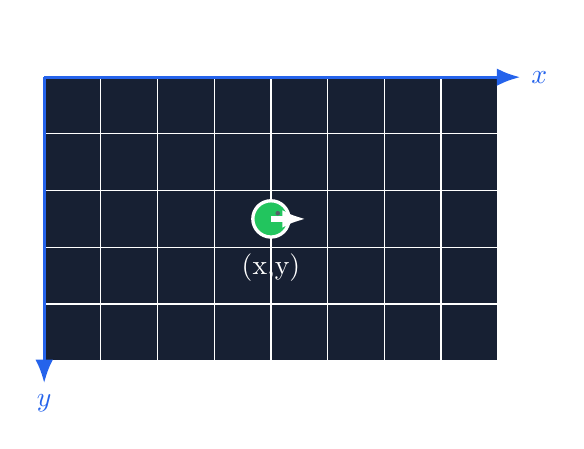
\begin{tikzpicture}[scale=0.72]
        \fill[Night] (0,0) rectangle (8,5);
        \draw[step=1, draw=white!12] (0,0) grid (8,5);
        \draw[Blue, line width=1.2pt, -{Latex[length=3mm]}] (0,5) -- (8.4,5) node[right] {$x$};
        \draw[Blue, line width=1.2pt, -{Latex[length=3mm]}] (0,5) -- (0,-0.4) node[below] {$y$};
        \node[white, anchor=south west] at (0.08,5.05) {(0,0)};
        \player{4}{2.5}
        \node[white] at (4,1.65) {(x,y)};
      \end{tikzpicture}
    \end{column}
    \begin{column}{0.4\textwidth}
      \begin{block}{Da ricordare}
        \begin{itemize}
          \item $x$ cresce verso destra.
          \item $y$ cresce verso il basso.
          \item ogni oggetto ha una posizione.
        \end{itemize}
      \end{block}
    \end{column}
  \end{columns}
\end{frame}

\begin{frame}[fragile]{Movimento = posizione + velocita'}
  \begin{lstlisting}[style=jsstyle]
let x = 80;
let velocitaX = 3;

function draw() {
  background("#172033");
  x = x + velocitaX;
  circle(x, 240, 70);
}
  \end{lstlisting}
  \vspace{0.25cm}
  
\begin{tikzpicture}
    \fill[Night] (0,0) rectangle (10.5,1.25);
    \foreach \x in {0.9,2.2,3.5,4.8,6.1,7.4,8.7} {
      \fill[Green] (\x,0.62) circle (0.18);
    }
    \draw[Yellow, line width=1.4pt, -{Latex[length=3mm]}] (0.9,0.25) -- (8.7,0.25);
    \node[white] at (5.2,1.0) {stessa regola, nuovo frame};
  \end{tikzpicture}
\end{frame}

\begin{frame}[fragile]{Una regola: rimbalza}
  \begin{lstlisting}[style=jsstyle]
if (x > width - raggio || x < raggio) {
  velocitaX = velocitaX * -1;
}
  \end{lstlisting}
  \vspace{0.15cm}
  \begin{block}{Traduzione}
    Se arrivi al bordo, vai nella direzione opposta.
  \end{block}
\end{frame}

\begin{frame}[fragile]{Input: il giocatore entra nel gioco}
  \begin{columns}[T]
    \begin{column}{0.6\textwidth}
      \begin{lstlisting}[style=jsstyle]
if (keyIsDown(LEFT_ARROW) || keyIsDown("a")) {
  player.x -= player.velocita;
}

if (keyIsDown(RIGHT_ARROW) || keyIsDown("d")) {
  player.x += player.velocita;
}
      \end{lstlisting}
    \end{column}
    \begin{column}{0.34\textwidth}
      \centering
      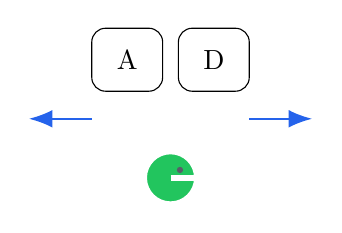
\begin{tikzpicture}
        \node[draw, rounded corners=5pt, minimum width=0.9cm, minimum height=0.8cm, fill=white] at (0,0) {A};
        \node[draw, rounded corners=5pt, minimum width=0.9cm, minimum height=0.8cm, fill=white] at (1.1,0) {D};
        \draw[Blue, thick, -{Latex[length=3mm]}] (-0.45,-0.75) -- (-1.25,-0.75);
        \draw[Blue, thick, -{Latex[length=3mm]}] (1.55,-0.75) -- (2.35,-0.75);
        \player{0.55}{-1.5}
      \end{tikzpicture}
    \end{column}
  \end{columns}
\end{frame}

\begin{frame}{Stato del giocatore}
  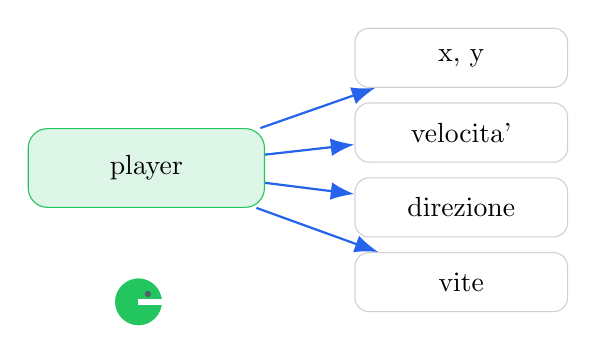
\begin{tikzpicture}[
    prop/.style={draw=Ink!20, fill=white, rounded corners=5pt, minimum width=2.7cm, minimum height=0.75cm, align=center},
    arr/.style={-{Latex[length=3mm]}, thick, draw=Blue}
  ]
    \node[draw=Green, fill=Green!15, rounded corners=7pt, minimum width=3cm, minimum height=1cm] (p) at (0,0) {player};
    \node[prop] (x) at (4,1.4) {x, y};
    \node[prop] (v) at (4,0.45) {velocita'};
    \node[prop] (d) at (4,-0.5) {direzione};
    \node[prop] (l) at (4,-1.45) {vite};
    \draw[arr] (p) -- (x);
    \draw[arr] (p) -- (v);
    \draw[arr] (p) -- (d);
    \draw[arr] (p) -- (l);
    \player{-0.1}{-1.7}
  \end{tikzpicture}
\end{frame}

\begin{frame}[fragile]{Array: una lista di proiettili}
  \begin{lstlisting}[style=jsstyle]
let bullets = [];

bullets.push({
  x: player.x,
  y: player.y,
  vx: player.dirX * 9,
  vy: player.dirY * 9
});
  \end{lstlisting}
  \vspace{0.15cm}
  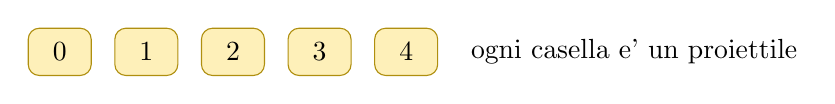
\begin{tikzpicture}
    \foreach \x/\i in {0/0,1.1/1,2.2/2,3.3/3,4.4/4} {
      \draw[fill=Yellow!30, draw=Yellow!70!black, rounded corners=4pt] (\x,0) rectangle ++(0.8,0.6);
      \node at (\x+0.4,0.3) {\i};
    }
    \node[right] at (5.5,0.3) {ogni casella e' un proiettile};
  \end{tikzpicture}
\end{frame}

\begin{frame}{Nemici: nascono fuori dallo schermo}
  \centering
  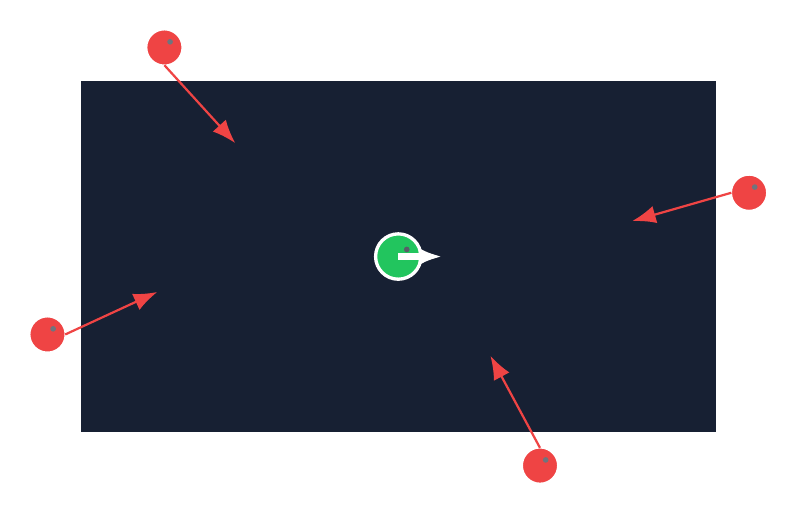
\begin{tikzpicture}[scale=0.9]
    \fill[Night] (0,0) rectangle (9,5);
    \draw[white, line width=1pt] (0,0) rectangle (9,5);
    \player{4.5}{2.5}
    \enemy{1.2}{5.45}
    \enemy{9.45}{3.4}
    \enemy{6.5}{-0.45}
    \enemy{-0.45}{1.4}
    \draw[Red, thick, -{Latex[length=3mm]}] (1.2,5.2) -- (2.2,4.1);
    \draw[Red, thick, -{Latex[length=3mm]}] (9.2,3.4) -- (7.8,3.0);
    \draw[Red, thick, -{Latex[length=3mm]}] (6.5,-0.2) -- (5.8,1.1);
    \draw[Red, thick, -{Latex[length=3mm]}] (-0.2,1.4) -- (1.1,2.0);
  \end{tikzpicture}
\end{frame}

\begin{frame}{Collisioni: quando due cerchi si toccano}
  \begin{columns}[T]
    \begin{column}{0.48\textwidth}
      \centering
      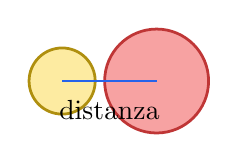
\begin{tikzpicture}[scale=1.2]
        \draw[fill=Yellow!40, draw=Yellow!70!black, line width=1pt] (0,0) circle (0.35);
        \draw[fill=Red!50, draw=Red!80!black, line width=1pt] (1.0,0) circle (0.55);
        \draw[Blue, line width=1pt] (0,0) -- (1,0);
        \node[below] at (0.5,-0.1) {distanza};
      \end{tikzpicture}
    \end{column}
    \begin{column}{0.47\textwidth}
      \begin{block}{Regola}
        Se la distanza tra i centri e' piu' piccola della somma dei raggi, c'e' collisione.
      \end{block}
      \[
        distanza < r_1 + r_2
      \]
    \end{column}
  \end{columns}
\end{frame}

\begin{frame}[fragile]{Collisione in codice}
  \begin{lstlisting}[style=jsstyle]
if (dist(bullet.x, bullet.y, enemy.x, enemy.y)
    < bullet.raggio + enemy.raggio) {
  bullets.splice(b, 1);
  enemies.splice(e, 1);
  score += 10;
}
  \end{lstlisting}
  \begin{block}{Qui succedono tre cose}
    il proiettile sparisce, il nemico sparisce, il punteggio sale.
  \end{block}
\end{frame}

\begin{frame}{Feedback: il gioco parla al giocatore}
  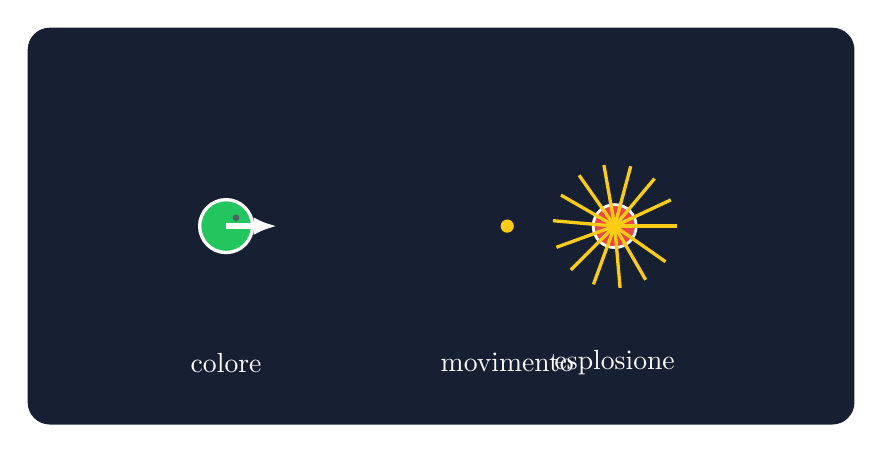
\begin{tikzpicture}[scale=1.05]
    \fill[Night, rounded corners=8pt] (0,0) rectangle (10,4.8);
    \player{2.4}{2.4}
    \enemy{7.1}{2.4}
    \foreach \a in {0,25,...,335} {
      \draw[Yellow, line width=1.2pt] (7.1,2.4) -- ++(\a:0.75);
    }
    \shot{5.8}{2.4}
    \node[white] at (2.4,0.75) {colore};
    \node[white] at (5.8,0.75) {movimento};
    \node[white] at (7.1,0.75) {esplosione};
  \end{tikzpicture}
\end{frame}

\begin{frame}{Mini shooter finale}
  \begin{columns}[T]
    \begin{column}{0.48\textwidth}
      \begin{block}{Cosa c'e' dentro}
        \begin{itemize}
          \item game loop;
          \item player controllato;
          \item sparo automatico;
          \item nemici che inseguono;
          \item collisioni;
          \item punteggio e vite;
          \item restart.
        \end{itemize}
      \end{block}
    \end{column}
    \begin{column}{0.48\textwidth}
      \centering
      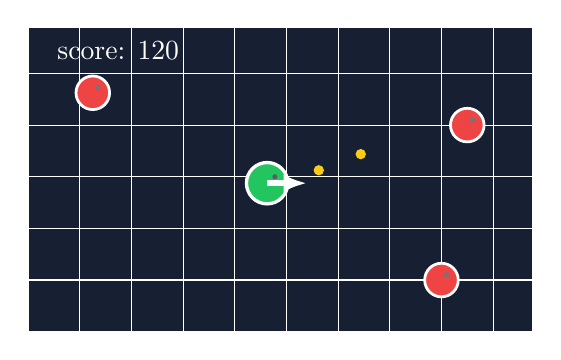
\begin{tikzpicture}[scale=0.82]
        \fill[Night] (0,0) rectangle (7.8,4.7);
        \foreach \x in {0,0.8,...,7.8} \draw[white!10] (\x,0) -- (\x,4.7);
        \foreach \y in {0,0.8,...,4.7} \draw[white!10] (0,\y) -- (7.8,\y);
        \player{3.7}{2.3}
        \enemy{1.0}{3.7}
        \enemy{6.8}{3.2}
        \enemy{6.4}{0.8}
        \shot{4.5}{2.5}
        \shot{5.15}{2.75}
        \node[white, anchor=west] at (0.3,4.35) {score: 120};
      \end{tikzpicture}
    \end{column}
  \end{columns}
\end{frame}

\begin{frame}{Domande per far ragionare}
  \begin{itemize}
    \item Che cosa succede se aumento la velocita' del player?
    \item Perche' i proiettili fuori dallo schermo vanno cancellati?
    \item Come potremmo aggiungere un boss?
    \item Come cambierebbe il gioco se i nemici scappassero invece di inseguire?
    \item Quale variabile controlla la difficolta'?
  \end{itemize}
\end{frame}

\begin{frame}{Sfide finali}
  \begin{columns}[T]
    \begin{column}{0.32\textwidth}
      \begin{block}{Facile}
        Cambia colori, dimensioni e velocita'.
      \end{block}
    \end{column}
    \begin{column}{0.32\textwidth}
      \begin{block}{Media}
        Aggiungi un nemico piu' lento ma piu' grande.
      \end{block}
    \end{column}
    \begin{column}{0.32\textwidth}
      \begin{block}{Difficile}
        Aggiungi power-up o livelli.
      \end{block}
    \end{column}
  \end{columns}
\end{frame}

\begin{frame}{Chiusura}
  \centering
  \Huge Un gioco e' un ciclo\\[0.25cm]
  \Large che legge input, aggiorna regole e disegna conseguenze.
  \vspace{0.5cm}

  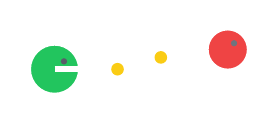
\begin{tikzpicture}
    \player{0}{0}
    \shot{0.8}{0}
    \shot{1.35}{0.15}
    \enemy{2.2}{0.25}
  \end{tikzpicture}
\end{frame}

\end{document}
